\documentclass[runningheads]{llncs}

\usepackage{graphicx}

\usepackage[automark]{scrlayer-scrpage}
\usepackage[T1]{fontenc}
% \usepackage{mathtools}
% \usepackage{amsfonts}
% \usepackage{amsmath}
\usepackage{tabu}
% \usepackage{amssymb,amsthm}
%\usepackage{stuki}
% \usepackage{tikz-uml}
\usepackage{geometry}
\usepackage{float}
\usepackage{diagbox}
\usepackage[utf8]{inputenc}
%%\usepackage[T1]{fontenc}
%%\usepackage[ttdefault=true]{AnonymousPro}
\usepackage{inconsolata}
\usepackage[T1]{fontenc}


\usepackage{listings}
%\usepackage{color}

\lstdefinelanguage{Clean}{%
    alsoletter={ABCDEFGHIJKLMNOPQRSTUVWXYZabcdefghijklmnopqrstuvwxyz_^`},%
    alsoletter={~!@\#\$\%^\&*-+=?<>:|\\.},%
   morekeywords={generic,implementation,definition,dynamic,module,import,from,while,then,else,where,in,of,case,let,infix,infixr,infixl,class,instance,with,if,derive,otherwise},%
%    otherkeywords={=,.,!,|,\&,\#,\\,=>,->,::,=:,\\\\,:==},%
    sensitive=true,%
    morecomment=[l]{//},%
    morecomment=[n]{/*}{*/},%
    morestring=[b]",%
    morestring=[b]',%
    emptylines=1,%
%    basicstyle=\scriptsize,%
    basicstyle=\small,%
%    identifierstyle=\sffamily,%
    identifierstyle=\ttfamily,%
    commentstyle=\itshape,%
    keywordstyle={\sffamily\bfseries},%
%    keywordstyle={\ttfamily\bfseries},%
    stringstyle=\ttfamily,%
    numbers=none,%
    showstringspaces=false,%
%    basewidth=0.50em,%
    basewidth=0.50em,%
    columns=[c]fixed,%
    keepspaces=true,%
    breaklines=false,%
%    breakindent=40pt,%
%    prebreak={\space...},%
%    postbreak={...\space},%
    tabsize=2,%
    texcl=true,%
    escapeinside={(\#}{\#)},%
    literate=   {\\}{{$\lambda$}}1%
                {A.}{{$\forall$}}1%
                {E.}{{$\exists$}}1%
                {<=}{{$\leq$}}1%
                {>=}{{$\geq$}}1%
                {<>}{{$\neq$}}1%
                {->}{{$\rightarrow$}}2%
                {|->}{{$\mapsto$}}2%
                {=}{{$=$}}1%
                {=>}{{$\Rightarrow$}}2%
                {<-}{{$\leftarrow$}}2%
                {==}{{${=\!\!\!=}$}}2%
                {=->}{{$\Rrightarrow$}}2%
                {==>}{{$\Longrightarrow$}}3%
%                {~}{{$\neg$}}1%
                {~~}{{$\approx$}}2%
                {~/~}{{$\ncong$}}2%
                {<~}{{$\lesssim$}}2%
                {</~}{{$\lesssim\!\!\!\!\!/\ $}}2%
                {\#}{{$\sharp$}}1%
                {\{|}{{$\!\{\!|$}}1%
                {|\}}{{$\,|\!\}$}}1%
                {<->}{{$\leftrightarrow$}}2%
                {<|>}{{$\updownarrow$}}2%
                {/.\\}{{$\wedge\!\!\!.\,$}}1%
                {/\\}{{$\wedge$}}1%
                {\\./}{{$\vee\!\!\!\cdot\,$}}1%
                {\\.n}{$\backslash$n}2%
                {\\n}{$\backslash$n}2%
                {\\"}{$\backslash$"}2%
                {\\t}{$\backslash$t}2%
                {\\\\t}{$\backslash$t}2%
                {\\\\}{$\backslash$t}1%
                {>>>}{{$>\!\!>\!\!>$}}2%
                {>>==}{{$>\!\!>==$}}5%
                {>>=}{{$>\!\!>=$}}3%
                {>>=.}{{$>\!\!>=\mathbf{.}$}}4%
%                {>>=.}{{$>\!\!>=\mathbf{.}$}}5%
                {:.}{{$:\!.$}}2%
                {***}{{$*\!\!*\!\!*$}}2%
                {\&\&\&}{{$\&\!\!\&\!\!\&$}}2%
                {<<<}{{$<\!\!<\!\!<$}}2%
                {\{|*|\}}{{$\{\!|\!\!\star\!\!|\!\}$}}3%
}%
%
\lstdefinestyle{numbers}{numbers=right, stepnumber=1, numberstyle=\tiny, numbersep=-7pt}
\lstnewenvironment{CleanCode}{\lstset{language=Clean}}{}%
\lstnewenvironment{CleanCodeN}{\lstset{language=Clean,style=numbers}}{}%
\lstnewenvironment{CleanCodeNB}{\lstset{language=Clean,style=numbers,frame=single}}{}%
\lstnewenvironment{CleanCodeB}{\lstset{language=Cleanframe=single}}{}%
%
\newcommand{\CleanInline}[1]{\lstinline[language=Clean]$#1$}%
\newcommand{\Cl}[1]{\lstinline[language=Clean]$#1$}%
\newcommand{\prog}[1]{\lstinline[language=Clean]$#1$}%

% \usepackage[dvips,usenames]{color}
% \usepackage[usenames]{color}
\usepackage{a0size}
\usepackage{times}
% \usepackage[latin2]{inputenc}
\usepackage{xcolor}
\usepackage{pgfplots}
%\usepackage{tikzscale}
\usepackage{listings}
\usepackage{caption}
\usepackage{multirow}
\usepackage{booktabs}
\usepackage{lipsum}
\usepackage{mwe}
% \usepackage{hyperref}
% \usepackage{breakurl}   
\usepackage{tikz}



% If you use the hyperref package, please uncomment the following line
% to display URLs in blue roman font according to Springer's eBook style:
% \renewcommand\UrlFont{\color{blue}\rmfamily}

\begin{document}
%
\title{Implementation of Digital Synthesis in Functional Programming\thanks{This work was supported by the European Union, co-financed by the European Social Fund, grant. no \textbf{EFOP-3.6.3-VEKOP-16-2017-00002.}}}
%
\titlerunning{Implementation of Digital Synthesis in Functional Programming}
% If the paper title is too long for the running head, you can set
% an abbreviated paper title here
%
\author{Evan Sitt \and Xiaotian Su \and Beka Grdzelishvili \and Zurab Tsinadze \and Zongpu Xie\\ Hossameldin Abdin \and Giorgi Botkoveli \and Nikola Cenikj \and Tringa Sylaj \and Vikt\'oria Zs\'ok \inst{\1}}
%
\authorrunning{E. Sitt et al.}
% First names are abbreviated in the running head.
% If there are more than two authors, 'et al.' is used.
%
\institute{E\"otv\"os Lor\'and University, Faculty of Informatics\\
Department of Programming Languages and Compilers\\
H-1117 Budapest, P\'azm\'any P\'eter s\'et\'any 1/C., Hungary\\
\email{\{sitt.evan, suxiaotian31, bekagrdzelishvili0, zukatsinadze, szumixie, hossamabdeen17, botko.gio, nicola.cenic, tringasylaj\}@gmail.com, zsv@inf.elte.hu}\\
-- Project Paper --
}

\maketitle


\begin{abstract}
Digital synthesis is a cross-discipline application used in fields such as music, telecommunication, and others. Digital synthesis involving multiple tracks, as well as parallel post-processes, lends itself naturally to the functional programming paradigm. The paper demonstrates this by creating a fully functional, cross-platform, standalone synthesizer application framework implemented in a pure lazy functional language. The application handles MIDI  input and produces WAV output played by any multimedia player.
Therefore, it can serve as a preprocessor for users who intend to create digital signals before transcribing them into digital or physical media.
Sufficient background and implementation techniques were explored for building software solutions for digital synthesis in functional programming. We demonstrate that functional programming concepts such as lazy evaluation using arrays are efficient for processing digital audio signals, and they are intuitive for working with music.

\keywords{Functional Programming  \and Digital Synthesis \and Waveforms \and MIDI \and WAV}
\end{abstract}

\section{Introduction}

\emph{Digital synthesis} is a \textit{Digital Signal Processing (DSP)}
technique for creating musical sounds. In contrast to \emph{analog synthesizers}\label{gloss:AnalogSythesizers}, digital synthesis processes discrete bit data to replicate and recreate a continuous waveform. 
The digital signal processing techniques used are relevant in many disciplines and fields 
including telecommunications, biomedical engineering, seismology, and others.
Digital synthesis is an application typically implemented in C++ with many frameworks provided \cite{maxiSynth,szanto}; however, their algorithms and methods are less intuitive.

Our project proposes to explore the applications of functional programming and to demonstrate 
its features in a framework implementation that can be used in multiple 
disciplines, such as broadcasting, mathematics education, physics education, application-oriented programming, and more.


Due to the parallel nature of processing multiple tracks of audio, the project is designed to replicate synthesis techniques by utilizing all the features and advantages of a purely lazy functional paradigm. While some algorithms were referenced, we implemented it from scratch. This is important as the algorithms that are used by typical frameworks are not made to be recursive, and as such, lack the optimizations from recursion. In addition, an algorithm built from scratch for a functional paradigm can avoid the many possible side effects that accompany the procedural algorithms.


In this paper, after briefly presenting a general background of digital synthesis (section 
\ref{sec:background}), the details of each project component are provided (section 
\ref{sec:project}). These include: intuitive description of the workflow (section \ref{sec:processflow}), diving into the explanation of the methods used for implementing the digital synthesis (section \ref{sec:wavetable}), clarification of amplitude modulation (section \ref{sec:envelope}), providing the details of the MIDI input file format (section \ref{sec:midi}), description of the methods used for processing the data (section \ref{sec:transcoding}) and finally analyzing the .WAV output file format (section \ref{sec:wav}).
These are, later on, followed by the summary of the results (section 
\ref{sec:Results}), by the related work (section 
\ref{sec:RelatedWork}), by the conclusions (section \ref{sec:Conclusion}), and by the
future plans (section \ref{sec:Further Work}).

\section{Background} \label{sec:background}

For understanding the basic idea behind the whole project, it is required to have basic mathematical knowledge about simple graph forms and graph manipulations, fundamental rules of sound generation and modification, as well as the principals and features of the functional programming paradigm. Knowing that the graph is defined as a visual representation of the dependency of a function's input value and result, the connection between it and functional programming is strong. The core graph feature used in this project is digital synthesis.
Digital synthesis is a field that was pioneered in the 1970s, and it is still continuously innovated by the music industry. Digital synthesizers\label{gloss:DigitalSythesizers} use the power of microprocessors to replicate analog synthesis. Among the techniques used are additive synthesis, \emph{wavetable lookup synthesis} (see subsection \ref{sec:wavetable} for details), and physical modeling.

Additive synthesis \label{gloss:additive} is a technique for creating \emph{waveforms} (see subsection \ref{waveform}) via the summation of sine waves. A sine wave is a waveform of pure single-frequency value. By summing multiple sine waves at various frequencies, amplitudes, and phase shifts\label{gloss:phaseShifted}, it is theoretically possible to generate all types of sound waves. The reference \cite{addSyn} gives more helpful information about this simple but commonly used concept, as a general base of generating sounds. Similarly, subtractive synthesis\label{gloss:subtractive} is a technique for creating \emph{waveforms} via the subtraction of sine waves.

Our application utilizes harmonic\label{gloss:harm} additive synthesis to create the basic waveforms commonly used to generate more complex synths. Harmonic additive synthesis involves using the Fourier series of a waveform to determine the weighted summation of sine waves to generate the target waveform. In other words, it is an expansion of those waves using their relationship and the concept of orthogonality. The usage of it is breaking up an arbitrarily long and periodical sequence into smaller, simple chunks that can be processed individually. Also, the Fourier series, when used with appropriate weights, can be used as a function approximator \cite{fourier}.  
These sine waves are called \textit{harmonics}, so-called because their frequencies are 
integer multiples of a standard fundamental frequency\label{gloss:freq}.

In order to generate the waveforms efficiently, digital waveform synthesis is typically implemented using wavetable lookup synthesis. 
In contrast to calculating a specific value of a waveform at a specific point of time, a waveform table is used to store one duty cycle of a waveform. The value of the waveform can be accessed by using the frequency to modify the access point of the waveform table and then multiplying by the appropriate amplitude. With this method, it is far more efficient to generate a waveform by use of constant time array access instead of repeated calculations. In section \ref{sec:wavetable}, the details of each waveform are given.

\section{Project details} \label{sec:project}

\subsection{The Process Flow from MIDI Input to WAV Output}
\label{sec:processflow}
As depicted in Figure \ref{fig:processflowdiagram}, the structure of the application's process flow is as follows:

\noindent \textit{MIDI Input:} 
        it opens the MIDI input file.
        Reads notation information and stores within a list.
        
\noindent \textit{Digital Signal Process Chain (DSP Chain):}
        it handles the signal generation and processing of the data.
        \begin{itemize}
            \item Sine Wavetable:
                The Sine Wavetable contains a hard-coded array of values corresponding to amplitude values of one cycle of a fundamental sine wave.
            \item Waveforms:
                Using the data of the wavetable and user-specified Fourier series, the Waveforms module does weighted summation to generate new waveforms.
            \item Envelope:
                Using an envelope profile, the Envelope module applies an ADSR envelope to the signal.
            \item Render:
                The final step of the DSP chain, the Render module generates signals from data passed from the MIDI Input module and outputs a final render for writing to file.
        \end{itemize}

\noindent \textit{Transcode:}
        it transcodes the render data into the proper encoding for 8, 16, or 32 bit PCM WAV format.
        
\noindent \textit{WAV Output:}
        it opens the WAV output file writes the transcoded render data to the final WAV output file.
%\end{itemize}

\begin{figure}[H]
	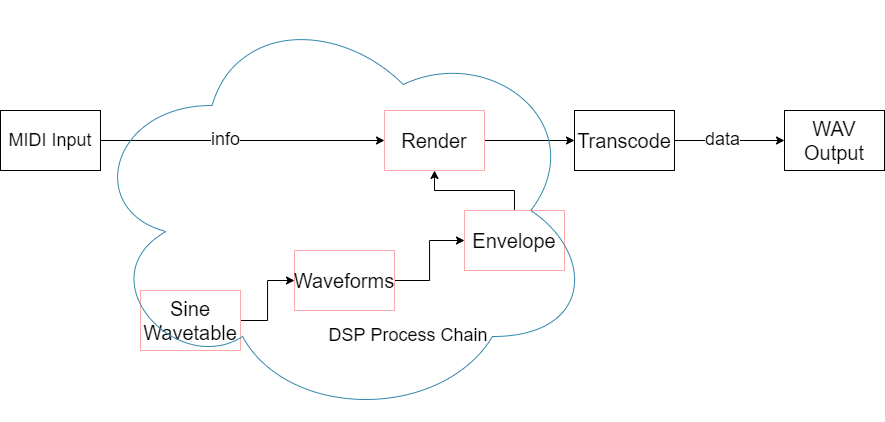
\includegraphics[width=1.0\textwidth, height=5.4cm]{process.png}
	\caption{The Signal Flow Modules}
	\label{fig:processflowdiagram}
\end{figure}

\subsection{Wavetable Lookup Synthesis} \label{sec:wavetable}

\subsubsection{Introduction}
In the early 1800s Fourier was able to prove that any periodic waveform is an infinite sum of so called frequency components, which are waveforms with single frequency having varying frequencies and amplitudes. This implies that any sound, no matter how complex can be built by using just sine waves, provided that correct frequency components are chosen. This fact became the foundation of a technique called \textit{Wavetable Lookup Synthesis}, in which a specific waveform is stored in a wavetable, and it exploits the relation between frequency and sampling rate to quickly build new waveforms. A waveform \label{waveform} is the shape of a signal's graph, which shows the changes in amplitude over a certain amount of time. Sine wave is the simplest of all waveforms and it contains only a single frequency and no harmonics, theoretically we can get any sound from waves, we can also write any program in binary, but of course we didn't do that. We used other simple waveforms (generated from the sine wave), as helpers, which will make building complex sounds much more straightforward.
We had to figure out how to sample from the stored wavetable and how to build new waveforms efficiently.
In the following section, we discuss our approach of making sampling wavetable as efficient as possible.

\subsubsection{Implementation}
Based on the methods for designing wavetables of \cite{organ}, our implementation chooses to set the size of the table as 2205, i.e., we store a table of 2205 real numbers, representing consecutive amplitudes within one single vibration of the sound wave. Thus, achieving the minimum sound intensity that humans can hear, which is 20 Hz.
The single cycle sine wavetable, shown in Figure \ref{fig:wavetable},
is the basis for our additive and subtractive synthesis\label{subractive}. As mentioned above, all the other waveforms can be efficiently generated from the sine wave by utilizing Fourier series \cite{additivesynth}. 

For each waveform, we generate a list of indices, which we need to sample from the wavetable, using the \Cl{getIndexes} function (listing \ref{cod:getIndexes}). These indices depend on the frequency and harmonic, and they are not necessarily integers.
The \Cl{getValues} function (listing \ref{cod:getV}) takes wavetable, frequency, harmonic, and duration as parameters, and it uses generated indices, while linear interpolation solves the complication caused by real indices.

\begin{lstlisting}[language=Clean,label={cod:getV},caption={Function \Cl{getValues}},captionpos=b]
getValues :: {Real} Frequency Int Samples -> [Real]
getValues waveTable frequency harmonic dur = [(getValue i waveTable) \\ i <- indexes]
where
    indexes = getIndexes frequency harmonic dur
\end{lstlisting}

\begin{lstlisting}[language=Clean,label={cod:getIndexes},caption={Function \Cl{getIndexes}},captionpos=b]
getIndexes :: Frequency Harmonic Samples -> [Real]
getIndexes frequency harmonic dur = map (\x = realRem x (toReal tableSize)) (take dur [0.0, rate..])
where
    newRate = toReal(SAMPLING_RATE)/((toReal harmonic)*frequency)
    rate = toReal(tableSize)/newRate
\end{lstlisting} 

The wavetable is implemented as an array. Even though lists offer much more functionality, they are actually linked-lists, and they do not give us access to the elements in constant time.

\begin{figure}[H]
        \centering
        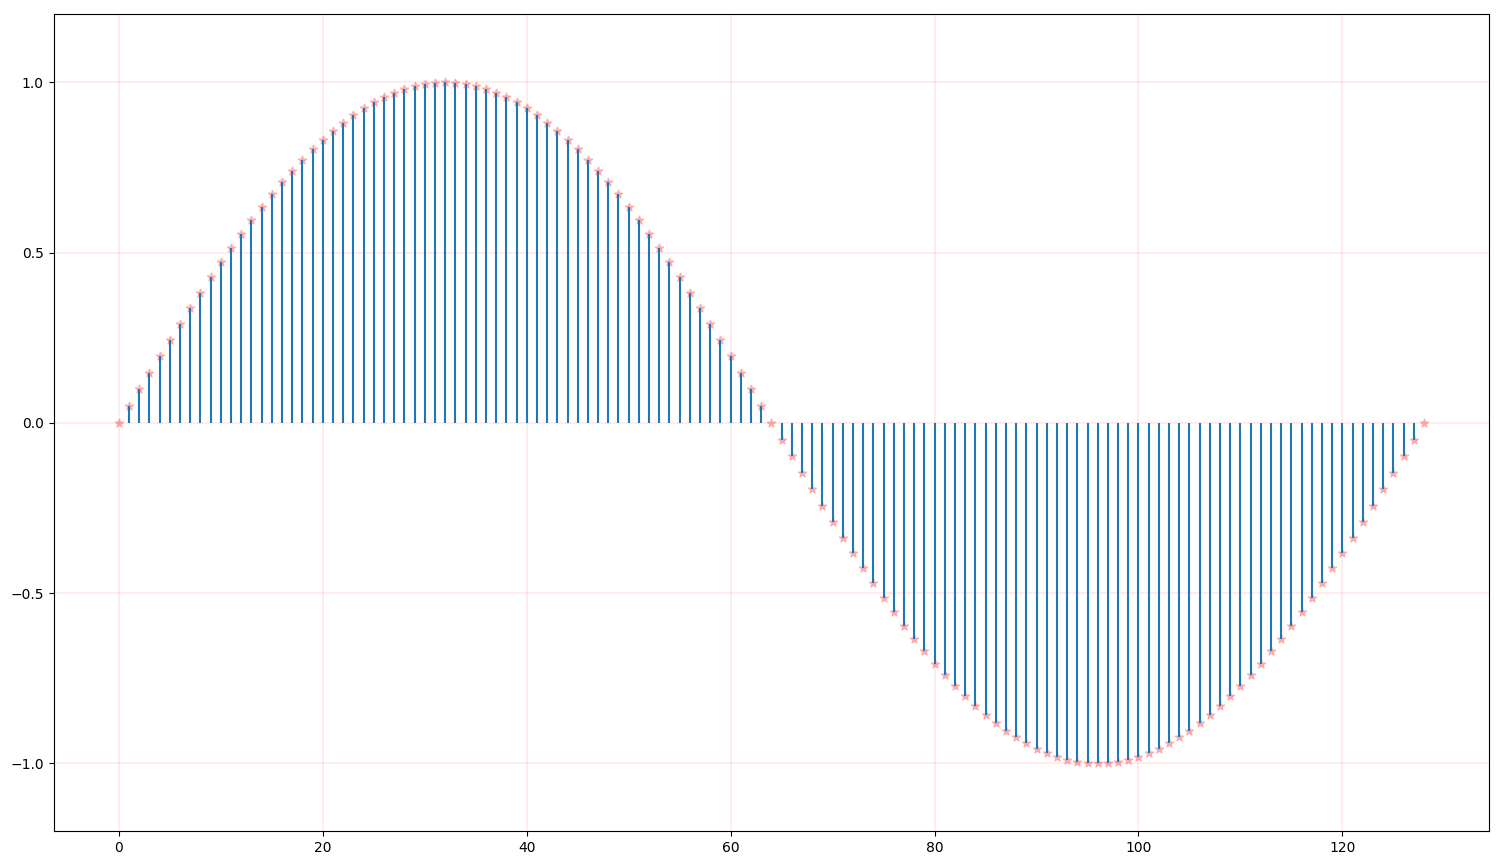
\includegraphics[width=\textwidth/2, height=3cm]{wavetable.png}
        \caption{Sine wavetable}
        \label{fig:wavetable}
\end{figure}

\subsubsection{Wave Forms}
Besides sine wave, we use square, triangle and sawtooth as our building blocks. The project also includes parameters to generate pulse, silence, and noise waves \cite{waveformRef}.
In the implementation, a waveform type is represented as an algebraic data structure: 

\begin{center}\Cl{:: Wave = Sine | Square | Triangle | Noise | Pulse | Sawtooth | Silence}\vspace{\baselineskip} 
\end{center} 

This is a parameter of our interface function, which generates waves as a list of \Cl{Real} numbers.
Each waveform has a list of harmonics and a list of amplitudes. In the case of square, triangle, sawtooth, and silence, these lists are easily defined, while for pulse and noise, there is a need for more sophisticated techniques, such as phase-shifting for noise and subtracting sawtooth wave from a phase-shifted version of itself for a pulse wave. Below you can see our graphical depictions of wavetables for each waveform.





%v what are these figure offering? relationships? typical usage situ of each?

\paragraph{\textbf{Sawtooth:}} Frequency components are all harmonics. Relative amplitudes are inverses of harmonic numbers and all 
harmonics are in-phase (see Figure \ref{fig:sawtooth}).

\paragraph{\textbf{Square:}} Frequency components are odd-numbered harmonics, relative amplitudes are inverses of the squares of the harmonic numbers, and all harmonics are in phase (see Figure \ref{fig:square}).

\begin{figure}[!htb]
    \centering
    \begin{minipage}{0.45\textwidth}
        \centering
        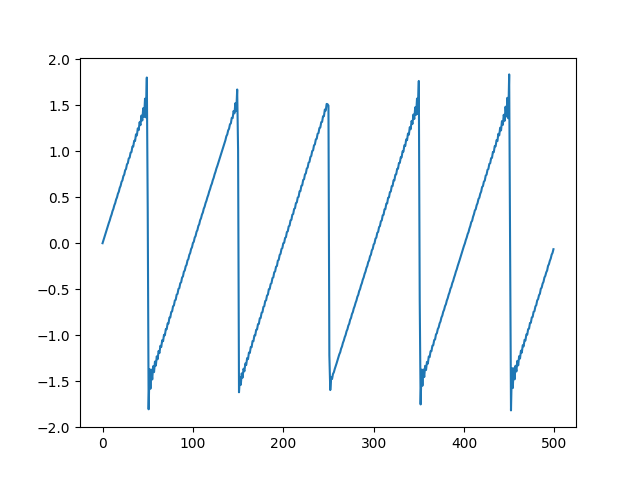
\includegraphics[width=0.9\textwidth,height=3.5cm]{saw.png}
        \caption{Sawtooth waveform}
        \label{fig:sawtooth}
    \end{minipage}
    \begin{minipage}{0.45\textwidth}
        \centering
        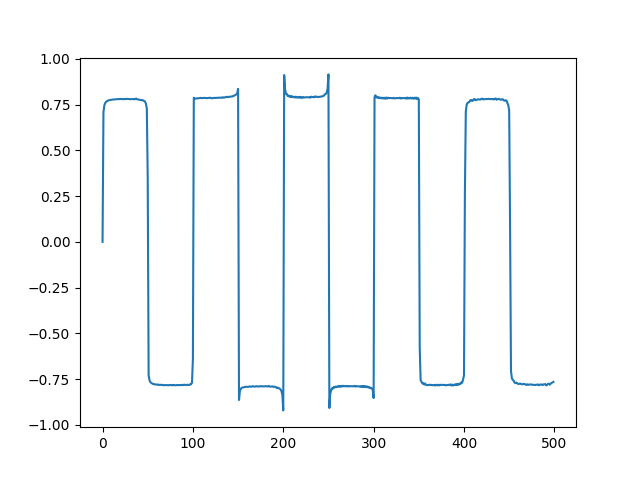
\includegraphics[width=0.9\textwidth,height=3.5cm]{square.png}
        \caption{Square waveform}
        \label{fig:square}
    \end{minipage}
\end{figure}

\begin{figure}[!htb]
    \centering
    \begin{minipage}{0.45\textwidth}
        \centering
        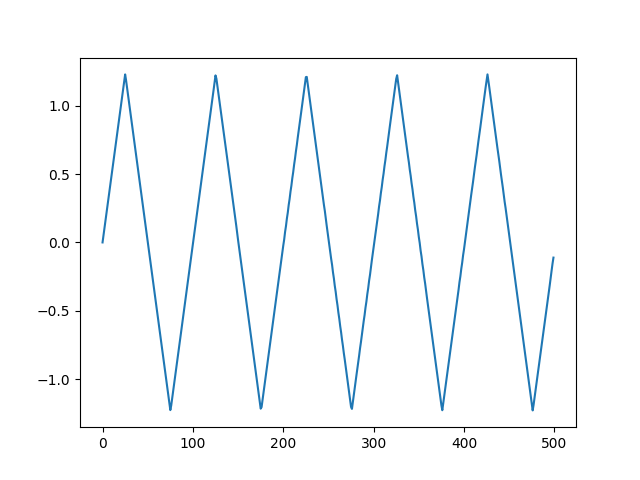
\includegraphics[width=0.9\textwidth, height=3.7cm]{triangle.png}
        \caption{Triangle waveform}
        \label{fig:triangle}
    \end{minipage}
    \begin{minipage}{0.45\textwidth}
        \centering
        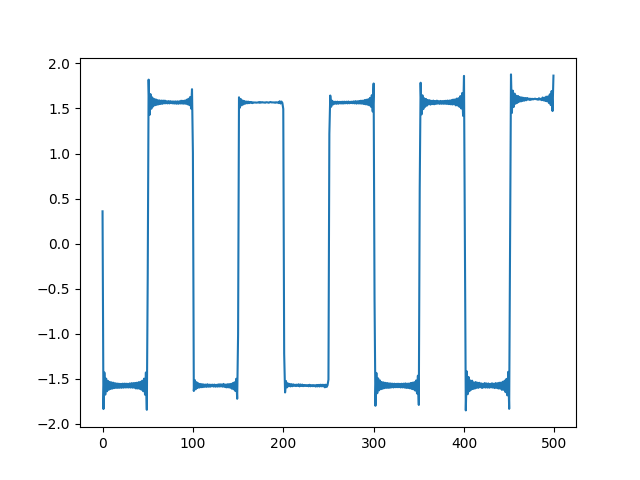
\includegraphics[width=0.9\textwidth,height=3.7cm]{pulse.png}
        \caption{Pulse waveform}
        \label{fig:pulse}
    \end{minipage}
\end{figure}

\paragraph{\textbf{Triangle:}} Frequency components are odd-numbered harmonics, relative amplitudes are inverse harmonic numbers and every second harmonic is 180 degrees out of phase (see Figure \ref{fig:triangle}).

\paragraph{\textbf{Pulse:}} For the Pulse wave generation, Figure \ref{fig:pulse}, Sawtooth wave, and phase-shifted version of itself are subtracted from it. For this, an efficient helper function, \Cl{shiftLeft}, is defined. It moves every element of a list by the given number to the left.  

\paragraph{\textbf{Noise:}} For generating the Noise wave, Figure \ref{fig:noise}, all amplitudes are equal to 1, and harmonics are random numbers. Again using the \Cl{shiftLeft} function, lists are shifted by a random number of places before summing them up. Clean provides functions to generate pseudo-random numbers using Mersenne Twister Algorithm \cite{randoms} in the module \Cl{Math.Random}.

\begin{lstlisting}[language=Clean,label={cod:harmonics_amplitudes},caption={Function that returns respective lists of harmonics and amplitudes for different waves}, captionpos=b]
harmonics_amplitudes :: Wave -> ([Real], [Real])
harmonics_amplitudes Sine = ([1.0],[1.0])
harmonics_amplitudes Sawtooth = ([1.0,2.0..50.0],[(-1.0)^(k+1.0)*(1.0/k) \\ k<-[1.0,2.0..50.0]])
harmonics_amplitudes Square = ([1.0,3.0..100.0],[1.0 / x \\ x <- [1.0,3.0..100.0]])
harmonics_amplitudes Triangle = ([1.0,3.0..100.0],
                     [(-1.0)^(i + 1.0) * (1.0/(k^2.0)) \\ k <- [1.0,3.0..100.0] & i <- [1.0..]])
\end{lstlisting}

\begin{figure}[!htb]
        \centering
        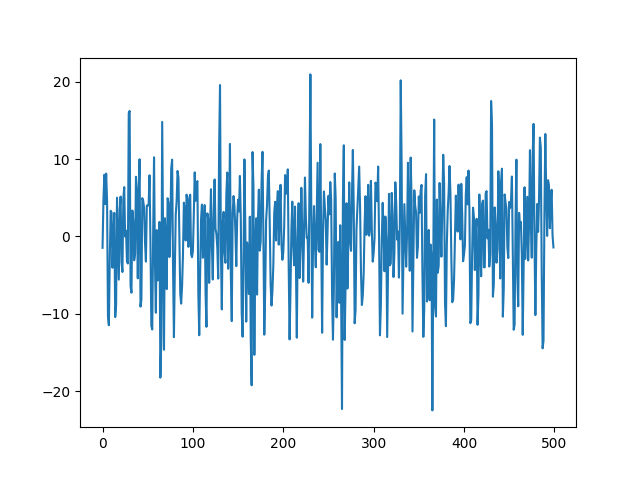
\includegraphics[width=0.7\textwidth,height=5cm]{noise.png} 
        \caption{Noise waveform}
        \label{fig:noise}
\end{figure}

\subsection{Envelopes} \label{sec:envelope}

\subsubsection{Introduction}
The data extracted from MIDI files are handled during rendering, Figure  \ref{fig:renderworkflow}. This process converts the given data to a sequence of numbers, which represents the sum of all waves after normalization. Before the summation, each wave should be modified using envelopes to get the actual sound of the musical instrument. In the music, an envelope describes the varying level of a sound wave over time. It is the envelope of a wave that establishes the sound’s uniqueness, and it has a significant influence on how we interpret music. Classic envelopes consist of 4 main parts: Attack\label{sec:envelopeStepsAttack}, Decay\label{sec:envelopeStepsDecay}, Sustain\label{sec:envelopeStepsSustain}, and Release\label{sec:envelopeStepsRelease}, where sustain refers to a level, while others represent time intervals. The attack is the period for which a sound needs to reach its peak from zero after the key is pressed. After the attack, the decaying period starts when the sound level decreases to sustain level and stays unchanged during the sustain phase until the key is released. The final phase of the envelope is the release, which continues until the sound fades to silence. Almost every musical instrument has its own individual envelope. For example, a quick attack with little decay makes a sound similar to an organ, while a longer decay is characteristic of a guitar. This application includes an envelope generator, which is a common feature of synthesizers and electronic musical instruments used to control the different stages of sound.

\subsubsection{Challenges}

\paragraph{\textbf{Starting value for Release:}} The release is the trickiest part of the envelope, as it does not have a fixed starting value, and it needs to be calculated based on the time of the release of the key. The first implementation of the envelope generator function used \Cl{last}, a built-in function for lists, to calculate the base value of the release. As lists are represented as linked lists and do not have direct access to the element, the \Cl{last} function used a recursive approach, which resulted in \(O(N)\) time complexity and excessive use of memory.

\textit{Solution:} To avoid overfilling the heap, the release base value is calculated directly using constant time and memory. At first, we determine which step the generation was terminated, and then the value can be calculated directly according to it.

\paragraph{\textbf{Getting envelope value during summation:}} The final sequence of numbers, which represents the actual sound, is the result of summing up sequences, generated for each \Cl{NoteChunk}. In functional programming, list summation might result in excessive use of memory and processing power if not implemented carefully.

\textit{Solution:} The first solution stored generated sequences in lists, and before starting the summation, silent sequences of appropriate lengths were appended to each of them on both ends to make their lengths equal, which made summation more straightforward. The second solution stored generated sequences in arrays, which provide direct access to each element in constant time. After calculating the offset based on the starting time for each array, array comprehensions and lambda functions were used to sum them up into one sequence.

\paragraph{\textbf{Storing envelope specifications:}} Envelopes have several steps, each of them specified by rate and/or level, but as they are not common, no built-in data structures exist for them in Clean. Since the number of values needed to generate a single envelope is more than a few, and it can even be infinite for \Cl{GeneralEnvelope}, it is essential to manage these data efficiently.

\textit{Solution:} Data types were implemented for each form of an envelope, to store and pass the envelope specifications efficiently. For example, for \Cl{GeneralEnvelope}, \Cl{EnvLevel} and \Cl{GenEnv} data structures were created to store rate and level values for each step and release starting index. 

\subsubsection{ADSR Envelope}
The first type of envelope implemented at the beginning of the project is ADSR. It is the simplest form of an envelope, which provides good bases for other more complex types, which are introduced later. The \Cl{getADSR} function is used to generate an ADSR envelope, Figure \ref{fig:adsr}. It has only four basic steps: Attack, Decay, Sustain, and Release. This function gets a beat\label{gloss:beat}, time signature, tempo\label{gloss:tempo}, and ADSR record as parameters. At first, the beat, time signature, and tempo are used to calculate the duration of the note, which is the time interval between pressing and releasing the key. \Cl{noteToSamples}, one of the utility functions, is used to convert these parameters to the number of samples in this time interval. After that, the number of samples for each step of the envelope is calculated.

Since the release is independent of the note duration, it is enough to convert the given release duration to samples directly, but the other three steps need different approaches. Instead of directly using the given duration of each step independently, the number of samples is calculated based on the time offset from the starting time and subtracting the sum of samples of the previous steps (As sustain does not have a fixed time interval, the total note duration can be used as offset). This is important, as it avoids losing samples during flooring\label{gloss:Flooring} of real numbers, and it makes sure that the number of total samples is equal to the sum of each step’s samples. After calculating the list of samples, each step of the envelope is calculated independently using list comprehension. For the linear attack and decay, the value of the sample is instantly calculated using the index, the number of samples, and the final value. Concatenating these lists produces the entire envelope excluding the release tail, however as the key may be released any time during the first three steps, including attack or decay, it might be necessary to shorten it. The Clean built-in function \Cl{take} is used for extracting the exact amount of samples needed. Finally, the release tail list is generated in the same way as the attack and decay and is concatenated to the others to get a complete envelope.

\begin{lstlisting}[language=Clean,label={cod:adsr},caption={The \Cl{getADSR} implementation}, captionpos=b]
getADSR :: Beat TimeSignature Tempo ADSR -> [Real]
getADSR beat timeSig tempo adsr = shortenedEnv ++ [...\\ x <- [1,2..releaseSamples]]
where
	noteDur = noteToSamples beat timeSig tempo
	attackSamples = secondsToSamples adsr.att
	decaySamples = (secondsToSamples (adsr.att+adsr.dec)) - attackSamples
	...
	wholeEnv = [1.0*((toReal x)/(adsr.att * (toReal SAMPLING_RATE))) \\ 
	           ...
	           ++ [adsr.sus \\ x <- [1,2..sustainSamples]]
	shortenedEnv = take noteDur wholeEnv
	endValue | noteDur == 0 = 0.0
			 | noteDur <= attackSamples = 1.0*((toReal (noteDur))/(adsr.att * (toReal SAMPLING_RATE)))
			 ...
			 = adsr.sus  
\end{lstlisting}

\subsubsection{DAHDSR Envelope}

The \Cl{getDAHDSR} function generates another type of envelope, which has two more steps than the ADSR envelope: delay and hold. Delay is the time interval before the attack, when sound stays silent, while hold phase comes after the attack and indicates the duration of the sound maintaining its peak. The implementation is similar to \Cl{getADSR} function and data is stored as the \Cl{::DAHDSR} record, shown bellow (listing \ref{cod:dahdsr}). Each step is generated using list comprehensions, and they are concatenated. The whole envelope is generated, then we take its prefix to make sure that the key can be released at any time.

\begin{lstlisting}[language=Clean,label={cod:dahdsr},caption={The \Cl{DAHDSR} envelope record}, captionpos=b]
:: DAHDSR = { delay :: Real
            , attack :: Real
            , hold :: Real
            , decay :: Real
            , sustain :: Real
            , release :: Real
            }
\end{lstlisting}

\subsubsection{Casio, 8 step Envelope}

Casio, Figure \ref{fig:casio}, is a more modern type of envelope which allows more flexibility and a wide variety. It is different from the types mentioned above, like the ADSR envelope (Figure \ref{fig:adsr}), For each step, instead of providing duration and level, it has eight steps, described by rate and level values, where the level is the desired percentage to be reached at the end of the current phase, while rate denotes the percentage with which samples change per second. Rate and level pair make it possible for the same phase to be ascending or descending depending on the needs of the users. Implementation of the Casio envelope differs from the other two envelopes, as the structure is different. The \Cl{CasioCZ} record provides data necessary for creating a Casio envelope. It has rate and level values for each of the eight steps. The first five steps represent the front part of the envelope, while the last three steps are used to generate the release tail after sustain. The \Cl{generateLine} function is used to generate point values of a line between two levels using the current rate. This function returns not a list of points, but a tuple of the list and real value. The second return value plays an essential role in interpolation. The last value of the line may not have an integer index. Hence it cannot be included in the list. Due to the reason mentioned above, instead of directly using the previous endpoint as the beginning for the current line, we need to recalculate it based on the second value of the \Cl{generateLine} function using the formula: \(\mathrm{casio.level1-rt2*(snd\ line1)}\). In the end, similarly to other envelopes, we need to take the exact amount of samples according to the note duration.


\begin{figure}[!htb]
    \centering
    \begin{minipage}{0.45\textwidth}
        \centering
        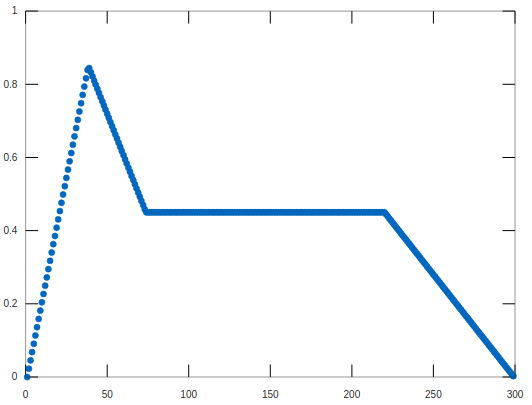
\includegraphics[scale=.25]{env1.png}
        \caption{ADSR envelope}
        \label{fig:adsr}
    \end{minipage}\hfill
    \begin{minipage}{0.45\textwidth}
        \label{env2}
        \centering
        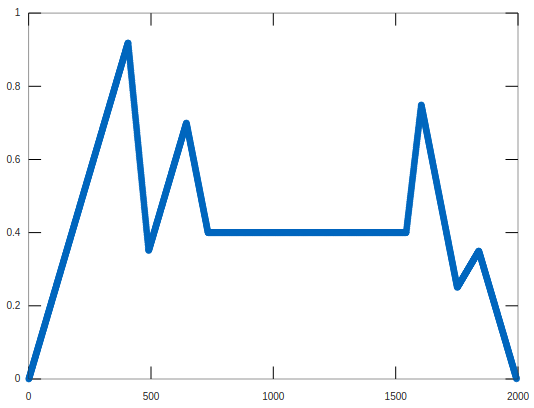
\includegraphics[scale=.25]{env2.png}
        \caption{8-Step Casio envelope}
        \label{fig:casio}
    \end{minipage}
\end{figure}

\subsubsection{Generalized Envelope}

The last type of envelope data structure is a Generalized Envelope, which is similar to Casio but provides even more flexibility during sound synthesizing. Both of them use rate and level values to describe each step, but generalized envelopes do not have a fixed number of steps like the other previous structures. The \Cl{GenEnv} record uses a list to store data, where each element is an \Cl{EnvLevel} record type, containing rate and level values. Also, as generalized envelopes do not have a fixed number of steps before the release tail, the \Cl{GenEnv} record contains a value for the index indicating sustain level. Generating data for each step is done similarly to the Casio envelope, but the rate and starting value cannot be recalculated manually, so data preprocessing is needed before using it. Therefore the implementation, which is shown below (listing \ref{cod:genenv}), is a bit different. \Cl{parseData} recursively traverses the initial list and generates a new one, which can be directly used to generate lines for each step using a similar method as in the Casio envelope.

\begin{lstlisting}[language=Clean,label={cod:genenv},caption={Generalized envelope generating function}, captionpos=b]
getEnvelope :: Real GenEnv -> [Real]
getEnvelope duration envelope = envShortened ++ envRelease 
where
    noteSamples = secondsToSamples duration
    sustL = toReal (hd [x.level \\ x <- envelope.levels &
                        d <- [1,2..(length envelope.levels)] | ind == envelope.sustainLevel])
    envIntroData = parseData (take envelope.sustainLevel envelope.levels) 0.0 0.0
    envIntro = [0.0] ++ (flatten [generateLine data \\ data <- envIntroData])
    envSustain = [sustL \\ x <- [1,2..(noteSamples-(length envIntro))]]
    envShortened = take noteSamples (envIntro ++ envSustain)
    envReleaseData = parseData (drop envelope.sustainLevel envelope.levels) 
                                (last envShortened) 0.0
    envRelease = flatten [generateLine data \\ data <- envReleaseData]
\end{lstlisting}

\subsubsection{Rendering waves and applying envelope} \label{rendering}

The rendering process consists of several steps. The first step is to calculate the whole length of the sound, as each wave can start at a different moment and can have distinct lengths. This value will be used later to generate a silent track, which will act as the base during the summing of all wave samples. The next step is to process data stored in each \Cl{NoteChunk} to generate sound waves and sum all of them up. Each \Cl{NoteChunk} stores wave type, time signature, tempo, envelope, and other data extracted from MIDI files, which are needed for generating wave and applying an envelope to it (Figure \ref{fig:modifiedsines}). Values for each wave can be calculated using already programmed functions for envelopes and sound synthesizing. After generating all the waves, we need to sum them up into a single list. If we use arrays, we can use each wave’s starting time as an index offset, but the same approach is not useful with lists. To easily sum up lists, they need to be the same size. Therefore the appropriate amount of silent samples should be appended on both sides of the list. Last step is normalization\label{gloss:normalization}: converting values to the \([-1.0, 1.0]\) range. After summing the lists up, some samples might go out of those bounds, which is why the final list needs to be normalized at the end of the process. After normalization, the sound rendering is finished, and it can be used for later processing.

\begin{figure}[!htb]
    \centering
    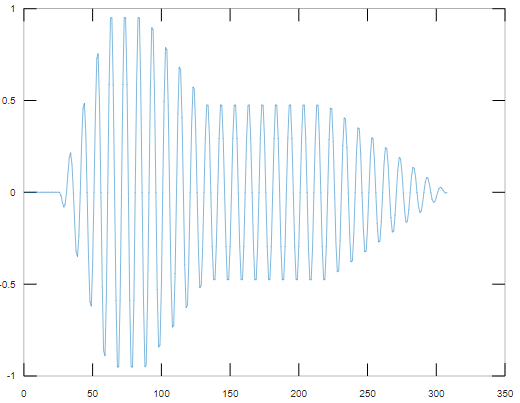
\includegraphics[scale=0.3]{sine1.png}
    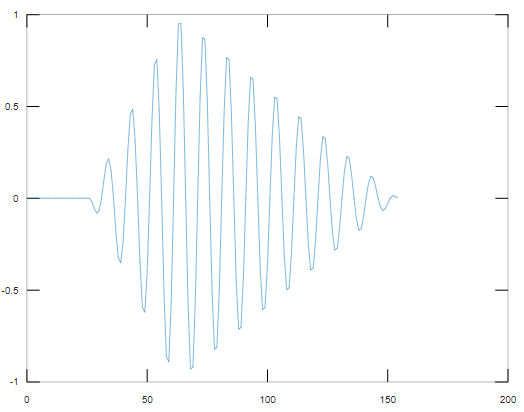
\includegraphics[scale=0.3]{sine2.png}
    \caption{Sine wave modified by different envelopes}
    \label{fig:modifiedsines}
\end{figure}

Four data structures were created to support different types of envelopes: ADSR, DAHDSR, Casio, and Generalized envelopes. A demonstration of DAHDSR followed by ADSR being applied to a sine wave is shown in Figure \ref{fig:modifiedsines}.
Several implementations were developed for this project, and the types of envelopes provide a flexible environment during music generation development and sound synthesizing. This variety of envelopes gives us the possibility to implement more efficient approaches during the rendering process and creating envelopes to generate more sophisticated and better sounds.
%v bib reference to these several implementations

\begin{figure}[!htb]
	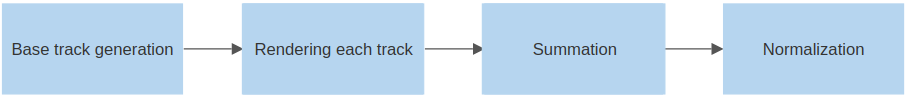
\includegraphics[width=1\textwidth,height=1.4cm]{renderingWorkflow.png}
	\caption{The workflow of rendering process.}
	\label{fig:renderworkflow}
\end{figure}

\subsection{MIDI Input}\label{sec:midi}
\subsubsection{General information about MIDI file} 

MIDI is short for Musical Instrument Digital Interface which is related to audio devices for playing, editing, and recording music. The MIDI file is just a stream of numbers, each of which is in the range from 0 to 255. The bytes order is big-endian\label{gloss:endianness}\label{gloss:big-endian} (as in \cite{midispec}).

MIDI files are the standard means of transferring MIDI data amongst users – it is a standard format across all computing platforms. MIDI files contain the standard channel-based MIDI messages, along with sequencer-related data (e.g., tempo, time and key signature, track names, etc.) and System Exclusive messages. Each message (also referred to as an event) is time-stamped.


Any decent MIDI sequencer should allow MIDI files to be loaded and saved, in addition to the use of any proprietary file format. MIDI files differ from most other types of music files in that they do not contain encoded sound (e.g., as in a WAV file). Consequently, compared with WAV or even MP3 files, MIDI files are extremely compact.

\label{gloss:chunk}
The content of a MIDI file is structured as a series of blocks of data referred to as chunks. Each chunk begins with a 4-character ASCII type. It is followed by a 32-bit length, most significant byte first. There are two main types of chunks defined in MIDI, as illustrated in the table below.
\label{gloss:header_chunk}
\renewcommand{\arraystretch}{1.0}
\begin{center}
	\begin{tabu}{|l|m{5em}|m{5em}|m{13em}|}
	   \hline
	   \diagbox[width=7.85em]{\bfseries type}{\bfseries structure}
	        & type \newline (4 bytes)
	        & length \newline (4 bytes) 
	        & data \newline (variable length of bytes) \\
		\hline
		Header Chunk & MThd & 6 & <format><tracks><division>\\ 
		\hline
		Track Chunk & MTrk & <length> & <delta\_time><events>... \\  
		\hline
	\end{tabu}
	\captionof{table}{Three types of MIDI Events}
\end{center}

\subsubsection{Information in MIDI file}The following introduces the most critical information in a MIDI file.

\noindent\textit{Format types of MIDI files}: This describes the chunk structure of a MIDI file and determines how the following MTrk chunks relate to one another (as in \cite{midisoft}).

    \begin{itemize}
     \item format 0: MIDI files, there should only be one MTrk chunk, and this can, therefore, contain any valid event - i.e., all timing-related and note (potentially multi MIDI channel) data.
     \item format 1: The first MTrk chunk is a global tempo track and should contain all timing-related events and no note data. The second and subsequent MTrk chunks contain the actual note data, and should not contain any timing related events. As all tracks are played together, they all follow the tempo map described in the global tempo track (the first MTrk chunk).
     \item format 2: Each track is a separate entity (like drum patterns within a drum machine), and can each contain any type of event. There is no global tempo track - each track may have its tempo map. Any timing-related events are specific to the track in which they occur.
    \end{itemize}
    
\paragraph{\textbf{tracks:}} Describe the number of track chunks contained in the MIDI file. Track chunks \label{gloss:track_chunk} (identifier = MTrk) contain a sequence of time-ordered events (MIDI and/or sequencer-specific data), each of which has a delta time value associated with it - i.e., the amount of time (specified in tickdiv units) since the previous event.

\paragraph{\textbf{delta\_time:}} The delta-time specifies the number of tickdiv intervals since the previous event (or from the nominal start of the track if this is the first event). If an event is to occur at the very start of a track, or simultaneously with the previous event, then it will have a delta-time of 0. The delta-time is a variable-length quantity in that it is specified using 1, 2, 3, or 4 bytes, as necessary.

\paragraph{\textbf{events:}} There are three main different kinds of events that can occur in track chunk; each type has a different number of bytes to store the information. We are not able to know the length of each specific event until we reach its status byte, which stores the information indicating what type it is.

\begin{itemize}
 \item Midi events (status bytes 0x8n - 0xEn)
Corresponding to the standard Channel MIDI messages, i.e., where 'n' is the MIDI channel (0 - 15). This status byte will be followed by 1 or 2 data bytes, as is usual for the particular MIDI message. Any valid Channel MIDI message can be included in a MIDI file.

 \item SysEx events (status bytes 0xF0 and 0xF7)
There are a couple of ways in which system exclusive messages can be encoded - as a single message (using the 0xF0 status), or split into packets (using the 0xF7 status). The 0xF7 status is also used for sending escape sequences.

 \item Meta events (status byte 0xFF) \label{MetaEvents}
These contain additional information that would not be in the MIDI data stream itself. E.g., TimeSig, KeySig, Tempo, TrackName, Text, Marker, Special, EOT (End of Track) events being some of the most common.
\end{itemize}
\renewcommand{\arraystretch}{1.0}
\begin{center}
	\begin{tabu}{|l|m{7em}|m{4em}|m{4em}|m{4em}|}
	    \hline
	    \diagbox[width=7.8em]{\bfseries event type}{\bfseries structure} 
	    & status byte & byte2 & byte3 & byte4 \\
        \hline
		MIDI events & 0x8n - 0xEn & data & (data) & $-$\\ 
		\hline
		sysex events & 0xF0 and 0xF7 & length & data & $-$\\  
		\hline
		meta events & 0xFF & type & length & data \\  
		\hline
	\end{tabu}
	\captionof{table}{Three types of MIDI Events}
\end{center}

\subsubsection{Challenges for parsing the MIDI file}
Unlike regular audio files like MP3 or WAV files, MIDI files do not contain actual audio data; therefore, it is much smaller in size. Due to this, they are more compact, but this makes it more difficult to parse it since there is much information to extract and store.
\subsubsection{Delta Time Issue}
Delta time is represented by a time value, which is a measurement of the time to wait before playing the next message in the stream of MIDI file data. Time values are stored as Variable-Length Values (VLV: a number with a variable width) \cite{vlv}. Each byte of delta time is consists of two parts: 1 continuation bit and 7 data bits. The highest-order bit is set to 1 if it needs to read the next byte, set to 0 if this byte is the last one in variable-length value.

\textit{Solution:}
To get an integer number represented by a  variable length value.
\begin{enumerate}
    \item convert the first byte in VLV to integer
        \begin{itemize}
            \item if it is greater than 128, put it into a list and read next byte recursively
            \item if not, just put this byte into a list and end the recursion
        \end{itemize}
    \item convert the list of bytes into one integer number
    \item return not only an integer of delta time but also the length of byte of it
\end{enumerate}

\subsubsection{MIDI Event Running Status Issue}
Different types of events already make it hard to parse information; in addition to that, the MIDI events use a data-thinning technique which is running status.
If the first (status) byte is less than 128 (hex 80), which implies that running status is in effect and that this byte is the first data byte (the status is carrying over from the previous MIDI event), this can only be the case if the immediately previous event is also a MIDI event because system exclusive events and meta events interrupt (clear) running status.

\textit{Solution:}
The length of the track chunk is useful since it does not only help for processing standard chunks but also makes it easier to deal with unexpected chunk types -- just by skipping that amount of bytes, then we can continue to process next chunk.

\subsubsection{Graphic Depiction of MIDI Processing} 

The following is a general structure of functions that deal with the information contained in MIDI file (see figure \ref{fig:midiprocess} and listing \ref{cod:process}).

\begin{figure}[!htb]
	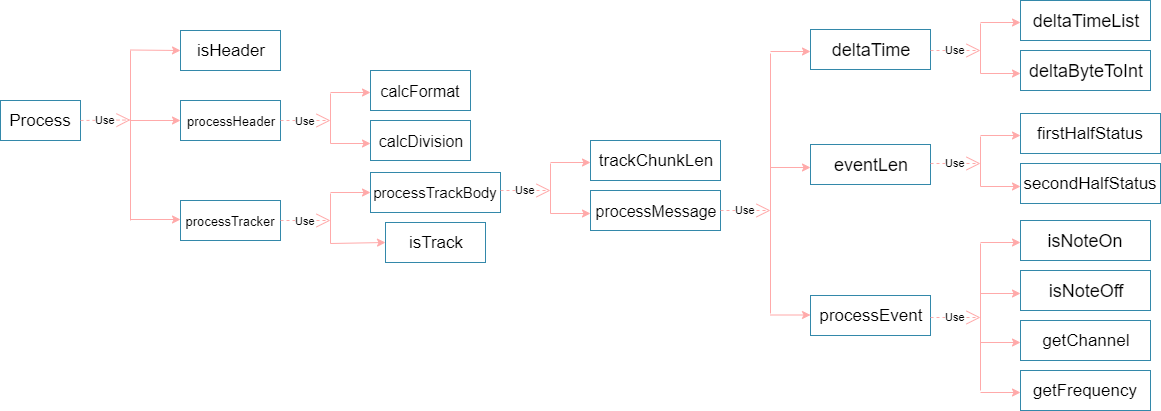
\includegraphics[width=1\textwidth,height=5cm]{functions.png}
	\caption{The MIDI processing functions}
	\label{fig:midiprocess}
\end{figure}

\begin{lstlisting}[language=Clean,label={cod:process},caption={The \Cl{process}, \Cl{processHeader}, \Cl{processTrack} functions}, captionpos=b]
process :: [Char] -> Info
process l | length l > 14 && isHeader (take 4 l) = { headerInfo = processHeader (drop 8 l), 
	                                                 trackInfo = processTrack (drop 14 l) }
	        = abort "not enough information"
	
processHeader :: [Char] -> HeaderInfo
processHeader l = { format = calcFormat (take 2 l), division = calcDivision (take 2 (drop 4 l)) }

processTrack :: [Char] -> [TrackInfo]
processTrack [] = []
processTrack l | isTrack l = processTrackBody (drop 4 l)
               = processTrackBody l
\end{lstlisting}

\noindent \Cl{process}: parses a MIDI file from scratch, accepting a list of Char (i.e., bytes) and returning an \Cl{Info} record, which contains information about header and track chunks. 

\noindent \Cl{isHeader}: takes the first four elements of a list of bytes and sees if it is the type of header chunk(\Cl{MThd}). The first six bytes of the list gives information about the format, the number of track chunks in total, and division. 

\noindent \Cl{processHeader}: stores the first and third value in the \Cl{HeadInfo} record.

\noindent \Cl{processTrack}: uses \Cl{isTrack} function to see if the beginning of a track chunk is currently being processed, and if so, it drops the first four elements which contain information of chunk type and continues processing the remaining information.

\subsection{Digital Sample Transcoding and Normalization}\label{sec:transcoding}


\subsubsection{General information about Transcoding} 
After the synthesis part, the signal needs to be converted into a form that can be recorded onto physical or digital media. This process is also known as \emph{transcoding}. In days of analogous signal synthesis, recording equipment transcoded the electrical signals using various mechanical or electromagnetic methods. With digital synthesis, the applications have to transcode the digital waveforms into bits in order to store them into the appropriate file. 

\subsubsection{Finding Suitable Form Challenge} Similarly to this concept, in this implementation, once the program obtains the wavetable examined in Section \ref{sec:wavetable}, the next step is to write this sound data to a WAV file.

As discussed in Section \ref{sec:wav}, three main components separate the WAV file: the \Cl{RIFF} chunk\label{gloss:RIFF}, the \Cl{fmt} sub-chunk and the \Cl{data} sub-chunk. The \Cl{data} sub-chunk contains the sound information, which is stored in bits. In consequence of that, it was necessary to find a way to convert the result of the wavetable into appropriate data for the file; hence there are transform functions implemented. 

\textit{Solution:} Initially, only the 8-bit version was created, which takes the list of output sample values and its maximum value and converts the values to fit the 8 bits range. In other words, the values of the samples are converted into an interval from 0 to 255. Later on, as a precondition for increasing the quality of the generated sounds, the function 16-bit version functionality was added, which alters the values to 16 bits samples stored into the interval 0 to $2^{16}-1$, and to maximize the quality of the generated sound 32-bit version, which alters the values to 32 bits samples stored into the interval 0 to $2^{32}-1$.

\subsubsection{Multiple Channels Challenge}
In a physical aspect, a \emph{channel}\label{gloss:channel} is the passage through which a signal or data is transported. In the case of audio files, it is the passage or communication channel in which a sound signal is transferred from the player source to the speaker. Since humans evolved to hear binaurally, in order to deliver more depth and spaciousness for enhancing the audio, then at least two channels are needed. That is why the creation of a multiple-channel version implementation was introduced as our next challenge.

\textit{Solution:} To make the project more flexible with the number of channels received input, two versions were made for the transform function. In the default case, the sound data obtained as the input will represent only one channel, meaning that the wavetable could be correctly represented as a list of Reals. On the other hand, in case the data has two or more channels, then a better representation would be a list of lists of Real. 

\subsubsection{Implemetation and Mathematical Background of Transcoding}
 After some research regarding the opportunities Clean offers and discussing the best technique possible, the best approach proved to be the concept of vertical graph shifting and multiplying. The most straightforward vertical graph transformation involves adding a positive or negative constant to a function, in other words, adding the same constant $k$ to the output value of the function regardless of the input shifts the graph of the function vertically by $k$ units. 

\begin{lstlisting}[language=Clean,label={cod:tf},caption={
The \Cl{transform\_one\_channel} function}, captionpos=b]
transform_one_channel :: [Real] Real BitVersion -> [Byte]
transform_one_channel list max bitVersion
= flatten (map (\x = toBytes Signed LE (translated_bit_version/BYTE_SIZE) x) 
(map (\x = moving_wave x max bitVersion) list))
    where translated_bit_version = translating_bit_version bitVersion
\end{lstlisting}
To give a more detailed explanation of the implementation(Listing~\ref{cod:tf}), it is a good idea to handle the 8, 16, and 32 bits cases separately. Regarding the 8 bit case, the first step is applying the \Cl{moving_wave} (Listing~\ref{cod:mv}) function to each element of the list.  When passing 8 as a \Cl{bitVerson} parameter, this function divides the number given with the \Cl{max}, which denotes the maximal possible value the input values from the given list can reach. In the case of real numbers from $[-0.5,0.5]$ this value is $0.5$. The next step is adding the \Cl{max} (0.5) and then multiplying each element by 255 ($2^8-1$) in order to get real numbers in $[0,255]$ interval . After that, the function \Cl{toInt} (build-in function in Clean) handles the conversion of the data from Real to Integer number, which concludes the moving process. The next step in the transformation is mapping the function \Cl{toBytes} that converts an Integer into a list of binary digits of length 8. The last thing done is flattening the list of Bytes into a list of bits that can be later written into the WAV file. If the input is a list of lists instead of a single list (in case of multiple channels), mapping the same transformation to every sub-list of the input does the proper conversion.

\begin{lstlisting}[language=Clean,label={cod:mv},caption={
The \Cl{moving\_wave} function}, captionpos=b]
moving_wave :: Real Real BitVersion -> Int
moving_wave targeted_number max bitVersion
| translated_bit_version == 8 = toInt(255.0*((targeted_number/(1.0*max)+0.5)))
= moving_wave_aux targeted_number max translated_bit_version
    where translated_bit_version = translating_bit_version bitVersion
moving_wave_aux :: Real Real Int -> Int
moving_wave_aux targeted_number max bitVersion
| targeted_number == max = 2^(bitVersion-1)-1
= floor((targeted_number*2.0^toReal(bitVersion-1))/max)
\end{lstlisting}
In the 16 bit case, when mapping the \Cl{moving_wave} instead of using \Cl{toInt} it was more appropriate to create the function \Cl{moving_wave_aux} which takes two real numbers (the number that  to convert (\Cl{targeted_number}) and the maximal possible value the numbers in the list can reach (\Cl{max})) and the Cl{bitVersion} (16) and returns $2^{15}-1$ if the \Cl{targeted_number} equals to \Cl{max} or otherwise the lower integer part of \Cl{targeted_number} multiplied by $2^{15}$ and divided by \Cl{max}. Following that, similar to the 8-bit version, the \Cl{toByte} mapping is performed. The transformation is concluded by just concatenating the sub-lists of bits of length 16 into a single list. If the input is a list of lists, mapping the same transformation to each sub-list of the input gives the expected output.

Similarly, on the 32-bit version, the first step is mapping \Cl{moving_wave}, which converts the input from a list of Real numbers to Integers, but now instead of working with $2^{15}$ the function mapped uses $2^{31}$. The following step is converting each integer into a list of bits of length 32 and, in the end, just concatenating all of the 32-length lists into one. If the input is given is a list of lists, handling it is done correspondingly to the 16-bit conversion.


\subsubsection{Evolution to the Interface}
As stated previously, initially, the implementation started with only one function, which covered the 8-bit case. Subsequently, in order to improve the quality of the sounds generated, the implementation was extended with two more functions corresponding to the 16-bit and 32-bit case. However, in time, it was established that the creation of an interface was much more generic, and hence more reliable. As observed before, the function \Cl{transform_one_channel} takes the bit version as a parameter, which makes it much more flexible in case further changes need to be introduced.

\subsection{WAV Output File Format} 
\label{sec:wav}

The WAV file is an instance of a \textit{Resource Interchange File Format} (RIFF) defined by IBM and Microsoft. Many audio coding formats are derived from the RIFF format (i.e., AVI, ANI, and CDR) \cite{wav}.
The most common WAV audio format is uncompressed audio in the linear pulse code modulation (LPCM). However, a WAV file can contain compressed audio, on Microsoft Windows, any Audio Compression Manager codec can be used to compress a WAV file. 

LPCM audio is a choice for professional users and audio experts in order to acquire maximum audio quality.
Beginning with Windows 2000, a \textit{WAVE FORMAT EXTENSIBLE} header was defined which 
specifies multiple audio channel data along with speaker positions, eliminates ambiguity 
regarding sample types and container sizes in the standard WAV format and supports defining 
custom extensions to the format chunk \cite{pcm}.

\subsubsection{The wav File Structure}

A RIFF file is a tagged file format. It consists of a specific container format called chunk, and the chunk has four character tag (FourCC)
and the size (number of bytes) of itself. The tag specifies how the data within the chunk should be interpreted, and there are several standard FourCC tags. Tags consisting of all capital letters are reserved tags. The outermost chunk of a RIFF file
has a RIFF form tag; the first four bytes of chunk data are a FourCC that specifies the form type and is followed by a sequence of subchunks. In the case of a WAV file, those four bytes are the FourCC WAVE. The remainder of the RIFF data is a sequence of chunks describing the audio information \cite{wav}.
The ability to extend the format later is a massive advantage for a tagged file format, as the mentioned format will not confuse the file reader. The rules of RIFF reader specifies that it should ignore all irrelevant tagged chunk and treat it as valid input. 

The chunk includes information as the title of the work, the author, the creation date, and copyright information. Some readers process the chunk as if it was the first in the RIFF form. On the other hand, other readers process as if it was a follower.
Attempts were made to make RIFF files for internationals use, so the CSET chunk was added to specify the country code, language, dialect, and code page for strings.
Junk chunk allows a chunk to be deleted, also has significant use since it allows the modification of the file without rewriting, by reserving some space.

The top-level definition of a WAV file is (as in \cite{wav}):

\begin{lstlisting}[language=Clean,label={cod:riffh},caption={RIFF header},captionpos=b]
<WAVE-form> -> RIFF('WAVE'
                    <fmt-ck>            // Format
                    [<fact-ck>]         // Fact chunk
                    [<cue-ck>]          // Cue points
                    [<playlist-ck>]     // Playlist
                    [<assoc-data-list>] // Associated data list
                    <wave-data> )       // Wave data
\end{lstlisting}

The definition has a few interesting points. The format chunk is necessary since it describes the format of the sample data that follows. The cue points chunk is optional and identifies some significant sample numbers in the wave file, the playlist and fact chunks are also optional. Finally, 
the mandatory wave data chunk contains the actual samples.
Unfortunately, the definition of the WAV file is foggy regarding the place of INFO chunk, as well as the CSET chunk, but the PCM format generated omits this chunk since the functionality does not depend on it. 

The WAV specification allows for not only a single, contiguous, array of audio samples, but also discrete blocks of samples and silence that are played in order. Most WAV files use a single array of data.

The specification for the sample data is confusing:
The \Cl{<wave-data>} contains the waveform data. It is defined as in the following \cite{wav}:
\begin{lstlisting}[language=Clean,label={cod:wavd},caption={Wave data},captionpos=b]
  <wave-data>  -> { <data-ck> | <data-list> }
  <data-ck>    -> data( <wave-data> )
  <wave-list>  -> LIST( 'wavl' { <data-ck> | // Wave samples
                                <silence-ck> }... ) // Silence
  <silence-ck> -> slnt( <dwSamples:DWORD> ) // Count of silent samples
\end{lstlisting}

In the wave data chuck (Listing \ref{cod:wavd}) produced by the application, the implementation changes \Cl{<data-list>} to \Cl{<wave-list>} in line 1 and \Cl{<wave-data>} to \Cl{<bSampleData:BYTE>} in line 2. These changes are done in order to avoid any possible recursion of \Cl{<wave-data>} contained in a \Cl{<data-ck>}. WAV files can contain embedded IFF \Cl{lists}, which can contain several \Cl{sub-chunks}.

\subsubsection{WAV File Format Limitation} 

The RF64 format specified by the European Broadcasting Union has been created to solve the limited file size issue of the WAV format since the WAV format can only handle files less than 4 GB because of its use of a 32-bit unsigned integer to record the file size header although this is equivalent to about 6.8 hours of CD-quality audio (44.1 kHz, 16-bit stereo). 

WAV format suffers from duplicated information between chunks. Also, 8-bit data is unsigned, which differs with 16-bits data which is signed, such inconsistency can be puzzling.
Based on the file specification of the WAV file format, a set of functions were implemented to create a framework for writing the data into a file. These functions have been enumerated in detail in the following pages.
In the process of making the framework for writing to a WAV file, we had to take into consideration some points, including the functional way in handling IO operations and language-specific features of Clean.

\subsubsection{Purity in Clean}
Due to Clean being a purely functional language, side effects such as
writing to a file is not as straightforward as in imperative languages.
Clean deals with this by using uniqueness typing to preserve referential
transparency \cite{clean}. Types which are marked as unique with
``\Cl{*}'' cannot be used multiple times for any path of the function
execution. It guarantees that at the time a function with unique
arguments is executed, the arguments have no more than one reference
pointed to each of them.
Clean uses the \Cl{World}\label{gloss:world} abstract type to represent the
environment or the state of the world in I/O operations. A program doing
I/O is given an environment and produces a new environment containing
the changes. A more complicated I/O program thus needs to chain the
subprograms together, bypassing the environment from one function to
another.

\subsubsection{Handling binary data in Clean}
The Clean \Cl{StdEnv} supports basic file manipulation in the
\Cl{StdFile} module. It provides operations for the \Cl{File} type,
which can also be a unique type.
%zuka can't understand following two lines
Opening a file requires an argument for a mode, which distinguishes read, write, and append, and between text files and binary data files. We used \Cl{FWriteData} mode for writing binary data.
There are several operations for writing data, though most of them are
not easy to work with for binary data. The smallest unit we can write is
%zuka can't understand difference between following two lines (done)
a \Cl{Char}. We assume a \Cl{Char} in Clean is a byte, we denote it with a type synonym as like \Cl{:: Byte :== Char}. %in Listing~\ref{cod:byte}.

\subsubsection{Writing byte sequences to file}
There is a function for writing a string (which are unboxed \Cl{Char}
arrays in Clean) to a file. However, lists are easier to work with most
of the time, so we defined a function to write a list of \Cl{Char}s
to a file as in Listing~\ref{cod:wbytes}.

The \Cl{!} in the type specifies that the arguments of the function are
strict, this can improve program efficiency in places where laziness is
not needed. \Cl{\#!} is a strict let notation, assigning the output
of \Cl{fwritec\ b\ f} to \Cl{f}. This \Cl{f} is not the same variable as
the \Cl{f} in the line before. It introduces a new scope and
shadows the previous variable. This use of name shadowing is encouraged in Clean with unique types as it makes the program somewhat resemble imperative programs, aside from the explicit passing of the unique file.
\begin{lstlisting}[language=Clean,label={cod:wbytes},captionpos=b,caption={Writing a list of bytes into a file}]
writeBytes :: ![Byte] !*File -> *File
writeBytes []     f = f
writeBytes [b:bs] f
  #! f = fwritec b f
  = writeBytes bs f
\end{lstlisting}


\subsubsection{Integer and byte conversion}
We need to manually define a function to convert a non-negative integer
to a list of bytes in \emph{little-endian}\label{gloss:lilEnd} order for later
use (Listing \ref{cod:tobytes}). It takes an argument that specifies
how many bytes the number should be represented, e.g., if the argument is 2, then the output will represent a 16-bit word, the rest of the number
is truncated. The function uses simple recursion and basic operators
from \Cl{StdEnv}. The first parameter is the number of bytes, and the second parameter is the integer to be converted.

\begin{lstlisting}[language=Clean,label={cod:tobytes},captionpos=b,caption={Converting an integer to a list of bytes}]
uintToBytesLE :: !Int !Int -> [Byte]
uintToBytesLE i n  | i <= 0 = []
                  = [toChar (n bitand 255) : uintToBytesLE (i - 1) (n >> 8)]
\end{lstlisting}

\subsubsection{Interface for writing a WAV file}
We implemented writing to a Wave file in (L)PCM format due to its
simplicity.
The type of the function for writing a Wave file is given in a
\Cl{dcl} file (definition module). It takes some parameters that
specify the structure of the file, and a list of bytes as the binary
data in the data chunk.
\begin{lstlisting}[language=Clean,label={cod:pcmdcl},captionpos=b,caption={Interface of writing a Wave file in PCM format}]
:: PcmWavParams = { numChannels    :: !Int // Number of channels
                  , numBlocks      :: !Int // Number of samples (for each channel)
                  , samplingRate   :: !Int // Sampling rate in Hz (samples per second)
                  , bytesPerSample :: !Int // Number of bytes in each sample
                  }
writePcmWav :: !PcmWavParams ![Byte] !*File -> *File
\end{lstlisting}

All data that the Wave file needs can be calculated from these
parameters. \Cl{numBlocks} represents the total number of blocks in
the data chunk, where each block contains \Cl{numChannels} samples.
\Cl{bytesPerSample} is how many bytes each sample contains.

\subsubsection{Implementation of writing a WAV file}
% TODO (done please check) implementation of what
The main function is composed of three smaller functions. The first one
writes the RIFF header into the file as in Listing~\ref{cod:wheader}.
\begin{lstlisting}[language=Clean,label={cod:wheader},captionpos=b,caption={Writing RIFF header into a file}]
writeHeader :: !Int !*File -> *File
writeHeader l f
  #! f = fwrites "RIFF" f
  #! f = writeUint 4 l f
  #! f = fwrites "WAVE" f
  = f
\end{lstlisting}

The first argument is the length of the whole file minus the first eight
bytes. It was calculated in the main function with 4 (the bytes
\Cl{WAVE}) + 24 (size of the format chuk) + 8 (header of the
data chunk) + \Cl{bytesPerSample} \(\times\) \Cl{numChannels}
\(\times\) \Cl{numBlocks} (size of the binary data) + (1 or 0
depending on whether the size of the bynary data is odd or even). \Cl{writeUint} is a utility function that combines \Cl{writeBytes} and \Cl{uintToBytesLE}.
The second function writes the format chunk, which contains writing in
the following data \cite{pcm}, using the same method as the previous function (Table~\ref{tab:fmt}).

%v resize the table - decrease row height (done)
\renewcommand{\arraystretch}{1.3}
\begin{table}[H]
\centering
\begin{tabu}{|c|c|X|}
\hline
Bytes & Value of the bytes               & \multicolumn{1}{c|}{Note}                                \\ \hline
4     & ``\Cl{fmt\ }''                   & The last byte is an space character                      \\ \hline
4     & 16                               & The size of the format chunk after the first eight bytes \\ \hline
2     & 1                                & This specifies the audio format to be PCM                \\ \hline
2     & \Cl{numChannels}                 &                                                          \\ \hline
4     & \Cl{samplingRate}                &                                                          \\ \hline
4 & \Cl{samplingRate} \(\times\) \Cl{bytesPerSample} \(\times\) \Cl{numChannels} & The amount of bytes processed per second \\ \hline
2 & \Cl{bytesPerSample} \(\times\) \Cl{numChannels}                              & The amount of bytes each block contains  \\ \hline
2     & 8 \(\times\) \Cl{bytesPerSample} & Bits per sample                                          \\ \hline
\end{tabu}
\caption{Data in the format chunk}
\label{tab:fmt}
\end{table}

The last function takes the length and the list of the binary data,
and writes it into the file using \Cl{writeBytes} after writing in
the chunk header. It also takes care of adding a padding byte if the
size of the data in bytes is odd.
The main function composes the smaller functions and evaluates the size
of the binary data so that it does not need to be calculated more than
once in the sub-functions (Listing~\ref{cod:wpcm}).
\begin{lstlisting}[language=Clean,label={cod:wpcm},captionpos=b,caption={The main function for writing Wave files}]
writePcmWav :: !PcmWavParams ![Byte] !*File -> *File
writePcmWav p d f
  #! l = p.bytesPerSample * p.numChannels * p.numBlocks
  #! f = writeHeader (l + if (isEven l) 36 37) f
  #! f = writeFormat p f
  #! f = writeData l d f
t  = f
\end{lstlisting}

After running a file through the function, a Wave file is
written, which can be played on a music player software.
The whole process can be seen in Figure~\ref{fig:writefile}.

\section{Results}\label{sec:Results}

%\subsection{Description of Outcome}
In the initial test runs of the application, we used a hard-coded notation of Beethoven's F\"ur Elise as input. The first 16 measures of F\"ur Elise was chosen as an initial test input as the notation involved only a single instrument, and the melodic and harmonic lines contained only monophonic lines. The initial test render of F\"ur Elise with only digital synthesis signals from the signal generation modules took a total amount of time ranging between 900 - 1000 seconds to complete. Further iteration on the application, in which the wavetable implementation was changed from lists to arrays, resulted in a subsequent rendering time of 4-6 seconds.

\begin{figure}[H]
\centering
\begin{tikzpicture}[scale=0.4]
\draw [rounded corners] (0,0) rectangle (22,-2);
\draw [rounded corners] (0,-4) rectangle (6,-6);
\draw [rounded corners] (8,-4) rectangle (14,-6);
\draw [rounded corners] (16,-4) rectangle (22,-6);
\draw [rounded corners] (-1,-8) rectangle (23, -10);

\draw [->, rounded corners, thick, blue] (-1,-1)
  -- (2,-1) -- (2,-5) -- (4,-5) -- (4,-1)
  -- (10,-1) -- (10,-5) -- (12,-5) -- (12,-1)
  -- (18,-1) -- (18,-5) -- (20,-5) -- (20,-1)
  -- (23,-1);

\node [above] at (11,-1) {\Cl{writePcmWav}};
\node [below] at (3,-5) {\Cl{writeHeader}};
\node [below] at (11,-5) {\Cl{writeFormat}};
\node [below] at (19,-5) {\Cl{writeData}};

\node [left] at (-1,-1) {\Cl{f :: File}};

\draw [->, thick, blue] (3,-6) -- (3,-9);
\draw [->, thick, blue] (11,-6) -- (11,-9);
\draw [->, thick, blue] (19,-6) -- (19,-9);

\node [below] at (11,-9) {Wave file};
\end{tikzpicture}
\caption{The process of writing a Wave file in Clean}
\label{fig:writefile}
\end{figure}

Following later implementation of the MIDI input and the Envelope modules, we were then able to do test renders using a variety of MIDI files. The first one we utilized was $simple.mid$, a MIDI file that the team created specifically to test the synth generation capacity of the program. $Simple.mid$ consisted of a series of A4 (440hz) notes at varying time intervals, from $1/16$ of a beat to a double beat. The design of $simple.mid$ was done to test the synth generation at different lengths of note values. Afterward, a sustained $CMaj$ chord is played to test the ability of the program to layer notes polyphonically.

The next MIDI file that we used to test the program with is $FurElise-Short.mid$. The MIDI file contains the first 16 measures of F\"ur Elise. For the same reason as the hardcoded version of F\"ur Elise, this MIDI file tests the program's capability to render two monophonic lines of melodic and harmonic content in parallel. The $FurElise.mid$ file is a MIDI file that extends this by containing the first 32 measures of F\"ur Elise. While the melodic and harmonic characteristics do not change much from the first 16 measures, the additional length of the track is a good test of complexity efficiency.



\renewcommand{\arraystretch}{1.0}
\begin{table}[H]
\centering
\begin{tabu}{|c|c|c|c|}
\hline
File Name  & Notes Read from File & Samples Rendered & Execution Time \\ \hline
simple.mid & 18 & 413083 & 2.87 \\ \hline
FurElise-Short.mid & 54 & 450923 & 10.32 \\ \hline
FurElise.mid & 298 & 2356043 & 296.24 \\ \hline
\end{tabu}
\caption{ Render time measurements }
\label{tab:results}
\end{table}

\section{Related Work}\label{sec:RelatedWork}

Euterpea \cite{euterpea} is a Haskell library for algorithmic MIDI
generation and low-level sound synthesis. Although it is written in a
purely functional language similar to our work, it heavily makes use
of functional reactive programming, which is a different approach
emphasizing interactivity, whereas we focus on music synthesis using
abstraction available in standard functional programming. The library also
comes with a textbook \cite{music} and a companion library that supports
real-time interactive applications.

Regarding Eric Zuubier's \cite{organ} work, similarities are obtained in the generation of music in Clean while using higher abstraction levels. Contrarily, this paper's implementation utilizes MIDI and WAV files for a more generalized digital synthesis, whereas Zuubier's work focuses on a more specialized digital synthesis for \emph{just intonation} (the tuning of musical intervals as whole number ratios of frequencies).\label{gloss:JustIntonantion}

Regarding Jerzy Karczmarczuk's work \cite{FuncFrameSynth}, there are definite similarities in the choice of the programming language as both applications are written in Clean, and both share the ability to handle multiple instruments. On the other hand, while we have a different approach in our implementation since we kept a high level of abstraction, Karczmarczuk uses a low-level of abstraction in his approach. Our approach places emphasis on a mathematical model; however, the physics and circuit like implementation were characteristic of Karczmarczuk's approach. Finally, while we were able to generate music, this was not done by Karczmarczuk's work \cite{FuncFrameSynth}.


Maximillian \cite{maxiSynth} is a C++ framework that is similar to our project in that it implements various waveform generators and envelopes. While we use similar techniques, the C++ implementation is optimized for the use of the procedural paradigm and live buffers while ours focuses on letting users create their waveforms via the Fourier series. Additionally, our implementations for envelope are far more intuitive to the actual sound design process.

\section{Conclusion}\label{sec:Conclusion}
The digital synthesizer application successfully demonstrated another major application of functional programming. There were some challenges in the process. These included: the creation of the framework for writing to WAV, the conversion of data to bit format, and the integration of the variety of specifications and conventions within the MIDI and WAV file formats.

The team was successful in implementing full-featured frameworks for importing MIDI files, writing to WAV files, and creating synths via additive synthesis\label, subtractive synthesis, and envelopes.


\section{Further Work}\label{sec:Further Work}

The application can be easily extended with further functionality to become more competitive with current offerings within the digital synthesis ecosystem. Support can be added for more import file types such as MusicXML and export file types such as .mp3, .flac, and 
.ogg.
Additional functionality can be added with filters based on frequency such as passes, shelves, and EQ, effects based on amplitude such as compression, gate, and distortion, and effects based on time such as delay, reverb, and chorus.

Lastly, adding support for live MIDI input, sample banks, VST3 support, and a graphical user interface will further bring the application in line with other digital synthesizers.


\bibliographystyle{splncs04}
\begin{thebibliography}{99}
\bibitem{cleanio} Achten, P., Plasmeijer, R.: The Ins and Outs of Clean I/O. \emph{Journal of Functional Programming}, 5(1), 81-110, 1995
\bibitem{addSyn} Additive Synthesis,
\url{https://www.soundonsound.com/techniques/introduction-additive-synthesis}
\bibitem{clean} Clean Language Report, \url{https://clean.cs.ru.nl/download/doc/CleanLangRep.2.2.pdf}
\bibitem{euterpea} Euterpea, \url{http://www.euterpea.com/}
\bibitem{fourier} Fourier Series,
\url{http://mathworld.wolfram.com/FourierSeries.html}
\bibitem{FuncFrameSynth} Functional Framework for Sound Synthesis,
\url{https://www.researchgate.net/publication/220802768\_Functional\_~Framework\_for\_Sound\_Synthesis}
\bibitem{midisoft} Guide to the MIDI Software Specification,
\url{http://somascape.org/midi/tech/spec.html}
\bibitem{music} Hudak, P., Quick, D.: Haskell School of Music -- From Signals to Symphonies,
\emph{Cambridge University Press}, 2018
\bibitem{pcm} Kabal, P.: Wave file specifications,
\url{http://www-mmsp.ece.mcgill.ca/Documents/AudioFormats/WAVE/WAVE.html}
\bibitem{maxiSynth} Maximilian: C++ Audio and Music DSP Library,
\url{https://github.com/micknoise/Maximilian}
\bibitem{randoms} Mersenne Twister Algorithm,
\url{http://www.math.sci.hiroshima-u.ac.jp/~m-mat/eindex.html}
\bibitem{wav} Microsoft and IBM Corporation, August 1991,
\url{https://web.archive.org/}
\bibitem{midispec} MIDI Files Specification,
\url{http://somascape.org/midi/tech/mfile.html}
\bibitem{additivesynth} Risset J.-C., Computer music experiments, \emph{Computer Music Journal}, vol. 9, no. 1, pp. 11–18, 1985
\bibitem{subSyn} Subtractive Synthesis, \url{https://www.musictech.net/guides/essential-guide/what-is-subtractive-synthesis/}
\bibitem{szanto} Szanto, G.: C++ Audio Library Options, \emph{Superpowered.com}, 2018,
\url{https://superpowered.com/audio-library-list}
\bibitem{thompsons} Thompson, S.: Haskell: The Craft of Functional Programming, 
\emph{ Addison-Wesley Professional}, 3rd edition, 2011
\bibitem{vlv} Variable Length Value,
\url{http://www.ccarh.org/courses/253/handout/vlv/}
\bibitem{waveformRef} What Are Waveforms And How Do They Work,
\url{https://soundbridge.io/what-are-waveforms-how-they-work/}
\bibitem{organ} Zuurbier, E.: Organ Music in Just Intonation, \url{https://www.ji5.nl/}
\end{thebibliography}

\section*{Glossary}
\textbf{\textit{additive synthesis}} (sec: \ref{gloss:additive}) - a sound synthesis technique based on adding waveforms together\\*
\textbf{\textit{analog synthesizer}} (sec: \ref{gloss:AnalogSythesizers}) - a synthesizer that uses analog circuits and signals to generate sound electronically\\*
\textbf{\textit{attack}} (sec: \ref{sec:envelopeStepsAttack}) - the period of time for which sound needs to reach peak loudness from zero, initiated by a noteOn event\\*
\textbf{\textit{beat}} (sec: \ref{gloss:beat}) - a standard of measurement to indicate relative time values of notes in relation to the time signature and tempo\\*
\textbf{\textit{big-endian}} (sec: \ref{gloss:big-endian}) - the most significant byte (the "big end") of the data is placed at the byte with the lowest address\\*
\textbf{\textit{channels}} (sec: \ref{gloss:channel}) - a channel is a set of audio data, each of which can be processed separately by an audio signal system\\*
\textbf{\textit{chunk}} (sec: \ref{gloss:chunk}) - a piece of data encoded into a MIDI file. There are two different types of chunks, the header chunk (sec: \ref{gloss:header_chunk}) and the track chunk (Reference: \ref{gloss:track_chunk}).\\*
\textbf{\textit{decay}} (sec: \ref{sec:envelopeStepsDecay}) - the period of time when the sound level decreases from the peak level to sustain level\\*
\textbf{\textit{digital synthesizer}} (sec: \ref{gloss:DigitalSythesizers}) - a synthesizer (electronic musical instrument that generates audio signals) that uses digital signal processing techniques to create musical sounds\\*
\textbf{\textit{endianness}} (sec: \ref{gloss:endianness}) - refers to the order of bytes (or sometimes bits) within a binary representation of a number. It can also be used more generally to refer to the internal ordering of any representation, such as the digits in a numeral system or the sections of a date.\\*
\textbf{\textit{flooring}} (sec: \ref{gloss:Flooring}) - function that takes as input a real number and gives as output the greatest integer less than or equal to the input\\*
\textbf{\textit{frequency}} (sec: \ref{gloss:freq}) - the number of waves that pass a fixed point in unit time\\*
\textbf{\textit{harmonics}} (sec: \ref{gloss:harm}) - is a signal or wave whose frequency is an integral (whole-number) multiple of a base frequency\\*
\textbf{\textit{just intonation}} (sec: \ref{gloss:JustIntonantion}) - the tuning of musical intervals as whole number ratios of frequencies\\*
\textbf{\textit{little-endian}} (sec: \ref{gloss:lilEnd}) - The least significant byte (LSB) value is at the lowest address. The other bytes follow in increasing order of significance. This is akin to right-to-left reading in hexadecimal order.\\*
\textbf{\textit{Meta events}} (sec: \ref{MetaEvents}) - events that occur within MIDI tracks and specify various kinds of information and actions, they may appear at any time within the track\\*
\textbf{\textit{MIDI}} (sec: \ref{sec:midi}) - is a protocol designed for encoding digital music instructions for digital music devices\\*
\textbf{\textit{normalization}} (sec: \ref{gloss:normalization}) - the level is changed to bring the highest PCM sample value or analog signal peak to a given level\\*
\textbf{\textit{phase-shifted}} (sec: \ref{gloss:phaseShifted}) - is the angle that the waveform has shifted from a certain reference point along the horizontal zero axis\\*
\textbf{\textit{release}} (sec: \ref{sec:envelopeStepsRelease}) - period of time until the sound fades to silence after a noteOff event\\*
\textbf{\textit{RIFF}} (sec: \ref{gloss:RIFF}) - Resource Interchange File Format - a generic file container format for storing data in tagged chunks\\*
\textbf{\textit{subtractive synthesis}} (sec: \ref{gloss:subtractive}) - is a sound synthesis technique based on subtracting one waveform from another\\*
\textbf{\textit{sustain}} (sec: \ref{sec:envelopeStepsSustain}) - period of time after the decay when the sound doesn't change until the key is released\\*
\textbf{\textit{tempo}} (sec: \ref{gloss:tempo}) - the speed at which a passage of music is or should be played\\*
\textbf{\textit{wav}} (sec: \ref{sec:wav}) - is an audio file format standard, developed by Microsoft and IBM\\*
\textbf{\textit{waveform}} (sec: \ref{waveform}) - a usually graphic representation of the shape of a wave that indicates its characteristics (such as frequency and amplitude)\\*
\textbf{\textit{wavetable}} (sec: \ref{sec:wavetable}) - a table of values representing a select portion of a sound wave\\*
\textbf{\textit{World}} (sec: \ref{gloss:world}) - an abstract type representing the environment, or the state of the world\\*
\end{document}
